%!TEX encoding = UTF-8 Unicode
\subsection{Related Computing Paradigms}
\label{sec:Computingparadigms}
\noindent In what concerns fog computing standardization, there is a lack of unanimity. As aforementioned, fog has been variously termed as cloudlets, edge computing, etc. Different research teams are proposing many independent definitions of fog (and fog-related computing paradigms). As there is a research gap in the definitions and standards for fog computing, this work follows the definitions that Ashkan Yousefpour et al. \cite{yousefpour2018all} present. Below, are described some paradigms that were raised in order to bring cloud closer to the end devices, as well as their pros and cons. As a conclusion, we show why fog computing is the natural platform for IoT.

\subsubsection{Mobile Computing}\label{subsec:MC}
\noindent Mobile/Nomadic Computing (MC) is characterized by the processing being performed by mobile devices (e.g., laptops, tablets, or mobile phones). It is necessary to overcome the inherent limitations of environments where connectivity is sparse or intermittent and where there is low computing power. As this model only uses mobile devices to provide services to clients, there is no need for extra hardware. They already have communication modules such as Bluetooth, WiFi, ZigBee, etc. As already mentioned, mobile devices have evolved in recent years. However, their resources are more restricted, compared to fog and cloud. This computing paradigm has the advantage of being characterized by a distributed architecture. The disadvantages of MC are mainly due to their hardware nature (i.e. low resources, balancing between autonomy and the dependency of other mobile devices; characteristic that prevails in all distributed architectures) and the need for mobile clients to efficiently adapt to changing environments \cite{satyanarayanan1996fundamental}. MC alone may not be able to meet the requirements of some applications. On the one hand, it is limited due to autonomy constraints and, on the order hand by low computational and storage capacity. This restricts the applications where this paradigm is feasible. For instance, it is unsuitable for applications that require low-latency and which, at the same time, generate large amounts of data that needs to be stored or processed. Nonetheless, MC can use both fog and cloud computing to enhance its capacities, not being restricted to a local network, expanding the scope of mobile computing and the number of applications where it can be used.

\subsubsection{Mobile Cloud Computing}
\noindent Cloud and fog computing, as mentioned in Section \ref{subsec:MC}, are key elements for validate the importance of MC. This interaction between them results in a new paradigm, called mobile cloud computing (MCC). MCC, differs from MC in the sense that mobile applications can be partitioned at runtime, so that computationally intensive components of the application can be handled through adaptive offloading \cite{shiraz2013review}, from mobile devices to the cloud. This characteristic increases the autonomy of mobile devices (i.e battery lifetime), as both the data storage and data processing may occur outside of them. Also, it enables a much broader range of mobile subscribers, rather than the previous laptops, tablets, or mobile phones. Unlike the resource-constrained MC, MCC has high availability of computing resources, scaling the type of applications where it is possible to use (e.g., augmented reality applications). Unlike MC, MCC relies on cloud-based services, where its access is done through the network core by WAN connectivity, which means that applications running on these platforms require connection to the Internet all the time. On the one hand, both MCC and MC suffer from the intrinsic characteristics of mobility, such as frequent variations of network conditions (intensified under rapid mobility patterns), and, on the other hand, even if the mobile devices remain fixed, MCC suffers from the inherent disadvantage of using cloud-based services (i.e. communication latency), which makes it unsuitable for some delay-sensitive applications with heavy processing and high data rate demands.

\subsubsection{Mobile Ad hoc Cloud Computing}
\noindent In some scenarios, there exists lack of infrastructure or a centralized cloud, so to implement a network based on MCC may not always be suitable. To overcome dependency on an infrastructure, Mobile Ad hoc Cloud Computing (MACC) was proposed \cite{hubaux2001toward}. It consists of a set of mobile nodes that form a dynamic and temporary network enabled by routing and transport protocols. These nodes consist of mobile ad hoc devices, which may continuously join or leave the network. In order to counteract the aforementioned characteristics inherent to this type of networks, and unlike MC, a set of ad hoc devices may form a local cloud that can be used in the network for purposes of storage and computation. Mobile Ad hoc NETworks (MANET), are imperative in use cases such as disaster recovery, car-to-car communication, factory floor automation, unmanned vehicular systems, etc. Although MANETs do not rely on external cloud-based services as MCC does, which mitigates the latency problem, it shares some limitations inherent to MC and ad hoc networks such as the power consumption constraints. Moreover, the formed local cloud may still be computationally weak and, as both network and cloud are dynamic, it is more challenging to achieve an optimal performance (i.e. as there is no infrastructure, mobile devices are also responsible for routing traffic among themselves).

\subsubsection{Edge Computing}
\noindent Edge Computing (EC), makes use of connected devices at the edge of the network to enhance its capabilities (i.e. management, storage, and processing power). It is located in the local IoT network, being ideally located one hop away from the IoT device and at most located a few hops away. Open Edge Computing defines EC as a computation paradigm that provides small data centers (edge nodes) in proximity to the users, enabling a dramatic improvement in customer experience through low latency interaction with compute and storage resources just one hop away from the user \cite{OpenEdge73:online}. As the connected devices don't have to wait for a centralized platform to provide the requested service, nor are so limited in terms of resources as in the traditional MC, their service availability is relatively high. Also, the restrictions over the autonomy are not so tight once there are not only mobile devices. Nonetheless, EC has some drawbacks. Latency, in this context, is composed by three components: data transmission time, processing time and result receiving time. Even though the communication latency is negligible, processing time may be significant. This computing paradigm only uses edge devices, whose computation and storage capabilities may still be poor (e.g., routers, switches), compared to fog or cloud computing, so this processing latency may still be too high for some applications.\\
\noindent\tab OpenFog Consortium states that fog computing is often erroneously called edge computing, but there are key differences between the two concepts \cite{OpenFog0208}. Although they have similar concepts, edge computing tends to be limited to the edge devices (i.e. located in the IoT node network), excluding the cloud from its architecture. Whereas, fog computing is hierarchical and it is not limited to a local network, but instead it provides services anywhere from cloud to \textit{things}. It is worth noting that the term edge used by the telecommunication's industry usually refers to 4G/5G base stations, Radio Access Networks (RANs), and Internet Service Provider (ISP) access/edge networks. Yet, the term edge that is recently used in the IoT landscape refers to the local network where sensors and IoT devices are located \cite{yousefpour2018all}.

\subsubsection{Multi-access Edge Computing}
\noindent Analogously, MCC is an extension of MC through CC, as Multi-access Edge Computing (MEC) is an extension of MC through EC (telecommunication's industry definition). ETSI defines MEC as computation paradigm that offers application developers and content providers cloud-computing capabilities and an IT service environment at the edge of the network. This environment is characterized by ultra-low latency and high bandwidth as well as real-time access to the radio network, that can be leveraged by applications \cite{ETSIMult81:online}. In MEC, operators can open their RAN edge to authorized third parties, allowing them to deploy applications and services towards mobile subscribers through 4G/5G base stations. The first approach to the edge of a network meant the edge of a mobile network, hence the name Mobile Edge Computing. As MEC research progressed, it was noticed that the term leaves out several access points that may also construct the edge of a network. This prompted the change from Mobile Edge Computing to Multi-access Edge Computing in order to reflect that the edge is not solely based on mobile networks \cite{MobileEd74:online}. Now it includes a broader range of applications beyond mobile device-specific tasks, such as video analytics, connected vehicles, health monitoring, augmented reality, etc. Similar to EC, MEC can operate with little to no Internet connectivity and use small-scale data centers with virtualization capacity to provide services. MEC is expected to benefit significantly from the up-and-coming 5G platform, as it allows for lower latency and higher bandwidth among mobile devices, and it supports a wide range of mobile devices with finer granularity.\\
\noindent\tab Both fog computing and MEC have the objective of offering similar type of features. Fog computing concentrates on applications, mainly IoT, that take advantage of a platform set that collectively assist end devices. MEC, on the other hand, focuses on application-related enhancements in terms of feedback mechanisms, information and content processing and storage, etc. \cite{taleb2017multi}.

\subsubsection{Cloudlet Computing}
\noindent Cloudlet Computing (cC) is another direction in mobile computing that aims to bring cloud closer to end devices through the use of cloudlets. M. Satyanarayanan et al. states that a cloudlet is a trusted, resource-rich computer or cluster of computers that is well-connected to the Internet and available for use by nearby mobile devices \cite{satyanarayanan2009case}. Cloudlet is, as the name suggests, a smaller sized cloud with lower computational capacity. It can be seen as a ``data center in a box'', where mobile users can exploit their VM to rapidly instantiate customized-service software in a thin client fashion. This way, it is possible to offload computation from mobile devices to VM-based cloudlets located on the network edge (telecommunication industry definition). Through those VMs, cloudlets are capable of providing resources to end devices in real-time over a WLAN network. The relatively low hardware footprint, results in moderate computing resources, but lower latency and energy consumption and higher bandwidth compared to cloud computing. The characteristics of this computing paradigm make it possible to handle applications with low-latency requirements, supporting real-time IoT applications. Y. Jararweh et al. \cite{jararweh2013resource} propose an architecture mobile-cloudlet-cloud, where they present three reasons which indicate that even though cloudlets are computationally powerful, they still need a connection to the cloud and its services: (1) heavy non real time jobs might be processed in the enterprise cloud while the real-time ones would be processed by the cloudlet, (2) accessing a file stored in the enterprise cloud, and (3) accessing some services that are not available inside the cloudlet. Although cloudlet computing fits well with the mobile-cloudlet-cloud architecture, fog computing offers a more generic alternative that natively supports large amounts of traffic, and allows resources to be anywhere along the cloud-to-things continuum. As it will be shown later, cloudlets are great resources and, in this way, they can be combined with the fog computing paradigm.

%muita coisa copiada, tentar reescrever
\subsubsection{Mist Computing}
\noindent Mist computing emerges to push IoT analytics to the ``extreme edge''. This computing paradigm is an even more dispersed version of fog. That means locating analytics tools not just in the core and edge, but also at the ``extreme edge'' \cite{Ciscopus95:online}. Mist computing layer is composed by mist nodes that are perceived as lightweight fog nodes. They are more specialized and dedicated nodes with low computational resources (e.g., microcomputers, microcontrollers) that are even closer to the end devices than the fog nodes \cite{iorga2018fog}. Therefore, mist computing can be seen as the first (non-mandatory) layer in the IoT-fog-cloud continuum. It extends compute, storage, and networking across the fog through the \textit{things}. This decreases latency and increases subsystems' autonomy. It can be implemented in order to enhance the services of predominance of wireless access and mobility support. The challenge with implementing mist computing systems lies in the complexity and interactions of the resulting network. These must be managed by the devices themselves as central management of such systems is not feasible.

\subsubsection{Concluding Remarks}
\noindent As was already mentioned, there are some other similar computing paradigms such as Follow Me Cloud (FMC), Follow Me Edge (FME), Follow Me edge-Cloud (FMeC) and Cloud of Things (CoT), to name a few. However, this state-of-the-art section had as first objective to investigate the most concepts addressed in the literature. The purpose was to understand their characteristics and to identify current limitations that must be tackled by novel solutions, in order to allow the deployment of delay-sensitive IoT systems in mobile environments. Table \ref{computing_paradigms} compares the features of the paradigms described above.\\
%Fig. \ref{computing_paradigms} shows a classification of the paradigms described above, as well as how they overlap in terms of scope.\\
\noindent\tab These computing paradigms present different pros and cons, having been proposed to cover different use cases. Even so, fog computing is suited for many use cases, including data-driven computing and low-latency applications, being the most versatile and comprehensive one. As aforementioned, fog is flexible enough to interact and take advantage of other paradigms such as edge, cloud, cloudlet and mist computing. Nonetheless, it may not be suitable for a few extreme use cases, such as disaster recovery or sparse network topologies where ad hoc computing (e.g., MACC) may be a better fit.
%\begin{figure}[t]
%	\centering
%	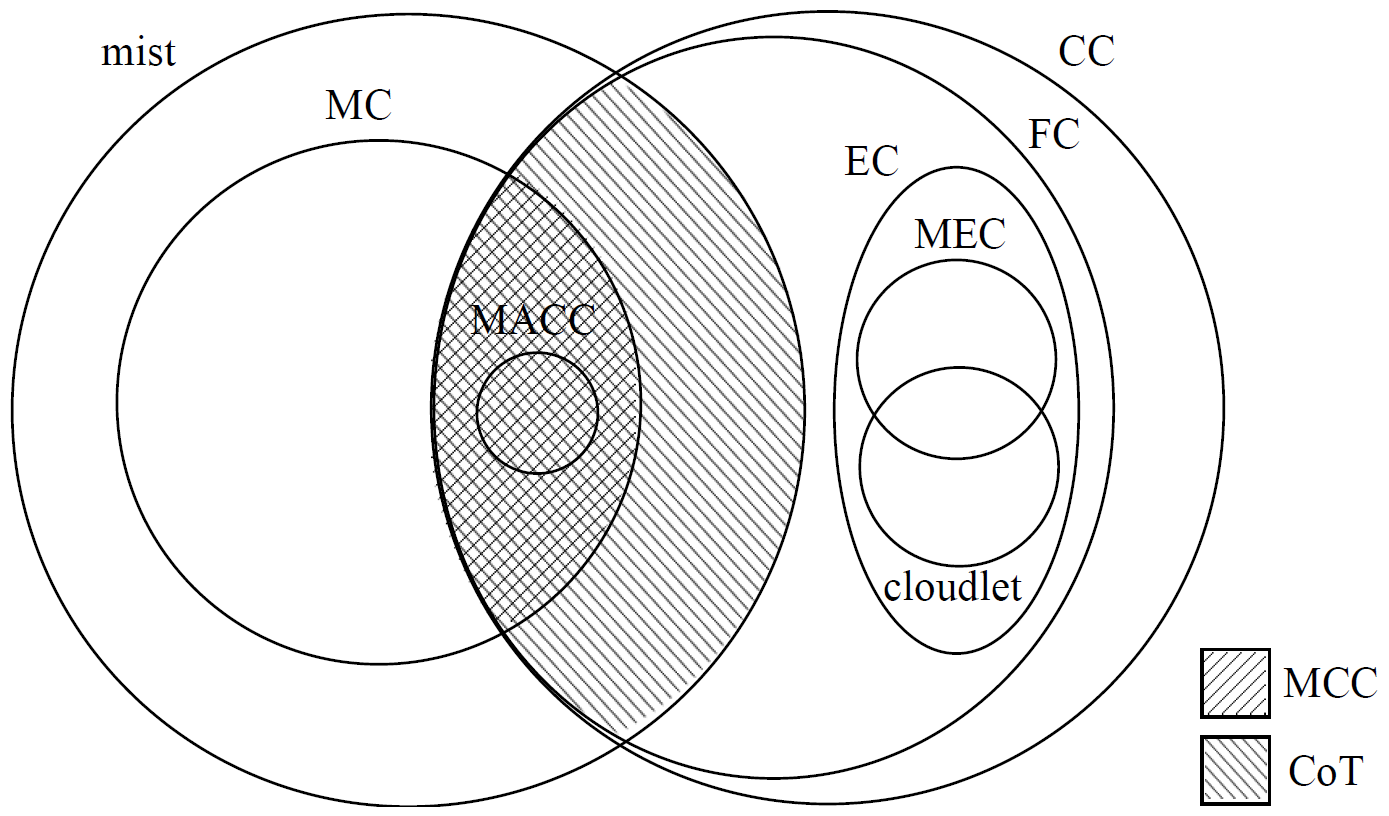
\includegraphics[width=80mm]{images/computing_paradigms}
%	\caption{A classification of scope of fog computing and its related computing paradigms (adapted from \cite{yousefpour2018all}).}
%	\label{computing_paradigms}
%\end{figure}
\begin{table}[!t]
	\scriptsize
	\begin{tabular*}{\textwidth}{l >{\centering\arraybackslash}m{0.4in} >{\centering\arraybackslash}m{0.4in} >{\centering\arraybackslash}m{0.4in} >{\centering\arraybackslash}m{0.4in} >{\centering\arraybackslash}m{0.4in} >{\centering\arraybackslash}m{0.4in} >{\centering\arraybackslash}m{0.4in} >{\centering\arraybackslash}m{0.4in} >{\centering\arraybackslash}m{0.4in}}
		\toprule
		\centering\textbf{Feature} & \textbf{CC} & \textbf{MC} & \textbf{FC} & \textbf{EC} & \textbf{MCC} & \textbf{MACC} & \textbf{MEC} & \textbf{cC} & \textbf{mist} \\[2pt]
		\toprule
		Heterogeneity support & \cmark &  & \cmark & \cmark & \cmark &  &  &  & \cmark \\ \midrule
		Infrastructure need & \cmark &  & \cmark & \cmark & \cmark &  & \cmark & \cmark & \cmark \\ \midrule
		Geographically distributed &  &  & \cmark & \cmark &  &  & \cmark & \cmark & \cmark \\ \midrule
		Location awareness &  & \cmark & \cmark & \cmark &  & \cmark & \cmark & \cmark & \cmark \\ \midrule
		Ultra-low latency &  &  & \cmark & \cmark &  &  & \cmark & \cmark & \cmark \\ \midrule
		Mobility support &  & \cmark & \cmark & \cmark & \cmark & \cmark & \cmark & \cmark & \cmark \\ \midrule
		Real-time application support &  &  & \cmark & \cmark &  &  & \cmark & \cmark & \cmark \\ \midrule
		Large-scale application support & \cmark &  & \cmark & \cmark &  &  & \cmark &  & \cmark \\ \midrule
		Standardized & \cmark & \cmark & \cmark & \cmark &  &  & \cmark &  &  \\ \midrule
		Multiple IoT Applications & \cmark &  & \cmark &  &  &  &  & \cmark & \cmark \\ \midrule
		Virtualization support & \cmark &  & \cmark &  &  &  & \cmark & \cmark &  \\ \bottomrule \\
	\end{tabular*}
	\caption{Features of fog computing related paradigms (adapted from \cite{yousefpour2018all}).}
	\label{computing_paradigms}
	\vspace{-5mm}
\end{table}